\section{PMNS model: global fits}
\label{sec:summary}


The large set of experimental results on neutrino oscillations, with the exception of the few anomalies that will be presented in section~\ref{sec:anomalies}, supports the global picture of three active neutrino mixing parametrized by the PMNS mixing matrix and the squared mass differences.

Global fits have been performed on the neutrino oscillation data by two groups~\cite{nufit,Capozzi:2016rtj} with results in good agreement.
The results of the most recent fit~\cite{nufit} are reported in Table~\ref{tab:globalfit} and in Fig~\ref{fig:globalfit} and in the following of this section.

\begin{table}[htbp]
\centering
\begin{tabular}{|c|c|c|}
  \hline
  Parameter & Normal Ordering & Inverted Ordering  \\ 
  \hline
$\theta_{12}$ (deg)& $33.56\:^{+0.77}_{-0.75}$ &  $33.56\:^{+0.77}_{-0.75}$\\  
  $\theta_{23}$ (deg)& $41.6\:^{+1.5}_{-1.2}$ &  $50.0\:^{+1.1}_{-1.4}$\\  
  $\theta_{13}$ (deg)& $8.46\:^{+0.15}_{-0.15}$ & $8.49\:^{+0.15}_{-0.15}$ \\  
  $\delta_{CP}$ (deg)&  $261\:^{+51}_{-59}$& $277\:^{+40}_{-46}$ \\  
  $\Delta m^2_{21}$ ($10^{-5}$eV$^2$)& $7.50\:^{+0.19}_{-0.17}$ & $7.50\:^{+0.19}_{-0.17}$ \\  
  $\Delta m^2_{3l}$ ($10^{-3}$eV$^2$)&  $2.524\:^{+0.039}_{-0.040}$&  -$2.514\:^{+0.038}_{-0.041}$\\  
  \hline
\end{tabular}
\caption{
PMNS parameters determined by a recent global fit to the world neutrino data \cite{nufit} in the hypothesis of normal ordering (second column) and inverted ordering (third column). The parameter $\Delta m^2_{3l}$ is equal to $\Delta m^2_{31}$ for NO and to -$\Delta m^2_{32}$ for IO. }
\label{tab:globalfit}
\end{table}


Presently, there is no significant preference for the normal or inverted ordering of the neutrino mass eigenstates. The measurement of the angles $\theta_{12}$ and 
$\theta_{13}$ and the mass squared differences $\Delta m^2 $ has already reached the few percent precision level. This is not the case for the angle $\theta_{23}$ where the three $\sigma$ range spans the interval (38,52) degrees (see also Fig.~\ref{fig:globalfit}) because of a mirror solution in the higher octant and the non-maximality of $\theta_{23}$ is not established. 
%It must be noticed that the fit reported in Table~\ref{globalfit} does not use the most recent Super-Kamiokande atmospheric results. 

The precise determination of $\theta_{23}$, of the CP-violating phase $\delta_{CP}$ and of the mass ordering remains a task for future experiments.

Another long standing feature of the underlying data is the 2 $\sigma$ tension between the determination of $\Delta m^2_{21}$ by KamLAND on one side, and the determination using the solar neutrino results by Super-Kamiokande, SNO and Borexino on the other side.
This tension is related to the non observation of the turn up on the lower part of the energy spectrum as predicted by the MSW effect. The observation of the day-night effect for solar neutrinos by Super-Kamiokande is also contributing to this tension.

The PMNS matrix, including all these measurements, has then this form~\cite{nufit}: 
\begin{equation}
|U| = \begin{pmatrix}
0.800 - 0.844 & 0.515 - 0.581 & 0.139 - 0.155 \\
0.229 - 0.516 & 0.438 - 0.699 & 0.614 - 0.790 \\
0.249 - 0.528 & 0.462 - 0.715 & 0.595 - 0.776 \\
\end{pmatrix}
\end{equation}
where the 3 $\sigma$ ranges for the magnitude of the elements are shown.
The Jarlskog invariant cannot be precisely determined today, however its maximum value, with the uncertainty at 1 $\sigma$, is 
\begin{equation}
J_{CP}^{max}
= 0.0329 \pm 0.0007 
\end{equation}
from Ref.~\cite{nufit}, to be compared to the Jarlskog invariant of the CKM matrix
$J_{CP}^{CKM} = (3.04 \: {}^{+0.21} _{-0.20} ) \times 10^{-5}$.

\begin{figure}[htbp]
\begin{center}
   	      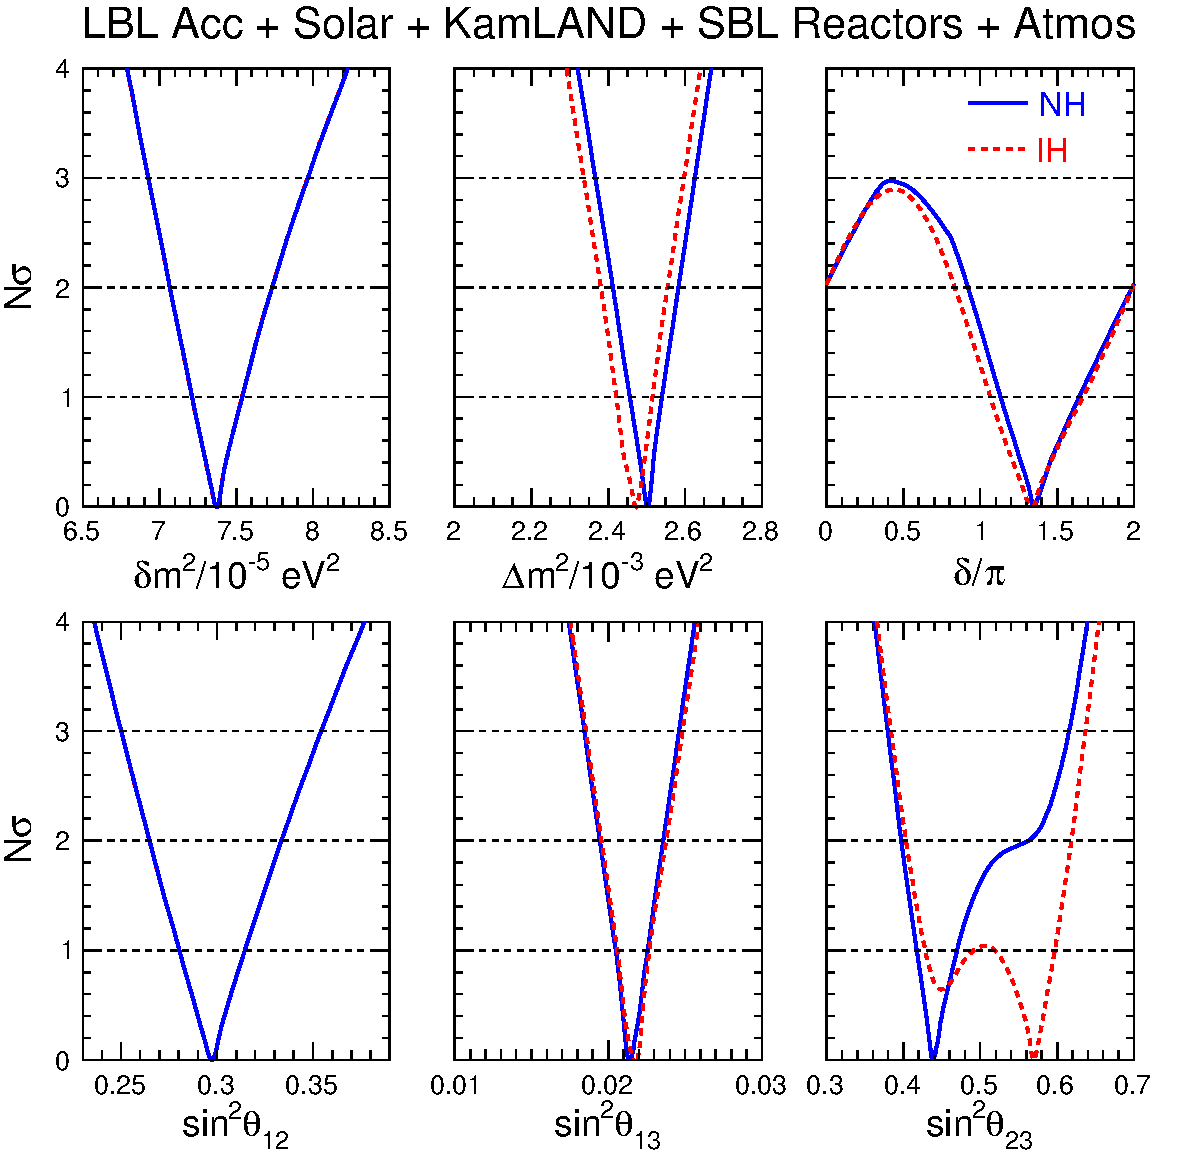
\includegraphics[width=0.8\linewidth]{figures/Fig_01_lisi.pdf}
    \caption{Bounds on the mass-mixing parameters in terms of
the number of standard deviations $\sigma$ from the best fit, for either normal ordering (solid lines) or inverted ordering (dashed lines)~\cite{Capozzi:2016rtj}. Bounds on \dmsqso and \thsol are
independent of the ordering. Horizontal dotted lines mark the 1, 2, and 3$\sigma$ levels for each parameter. The parameters $\delta m^2$ and $\Delta m^2$ are defined as 
$\delta m^2 = m^2_2 - m^2_1$ and $\Delta m^2 = m^2_3 - (m^2_2 + m^2_1)/2$.
This fit does not include the latest 2016 T2K results for $\delta_{CP}$.
Courtesy of F. Capozzi et al.}
 \label{fig:globalfit}
 \end{center}
\end{figure}


